\chapter*{Predicting Income}
\stepcounter{chapter}

\section{Value of Education}
\begin{figure}[H]
    \centering
    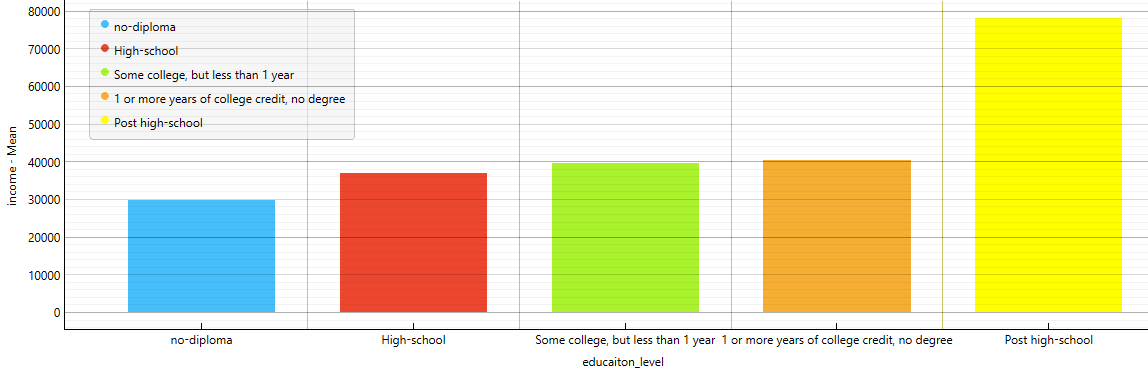
\includegraphics[width=0.8\textwidth]{chapters/part 3 - image/avg_income_edu.png}
    \caption{Average income with respect to education level}
    \label{fig:income_edu}
\end{figure}

\begin{table}[h]
    \centering
    \caption{Average Income by Education Level}
    \label{tab:income_edu}
    \begin{tabular}{l S[table-format=5.2]} % 5 digits before decimal, 2 after
        \toprule
        \textbf{Education Level} & {\textbf{Avg. Income (\$)}} \\
        \midrule
        No Diploma                & 30068.50 \\
        High School               & 37065.50 \\
        Some College (<1 year)    & 39678.80 \\
        College (1+ years but no degree)        & 40556.70 \\
        Post High-School          & 78343.00 \\
        \bottomrule
    \end{tabular}
\end{table}
Further supporting \ref{sec:education_section},
figure \ref{fig:income_edu} illustrates a clear positive correlation between educational attainment and average income.
Evaluating education on a year-by-year basis is problematic because time does not always equate to a standardised outcome or formal
accreditation. Value can vary between years, with final years (when you get a certification) forming income spikes. Current jobs may also
not be influenced by time in education due to experience or the fact that they may be overqualified.




\section{Predicting Income Bracket}
% node structure
\begin{figure}[H]
    \centering
    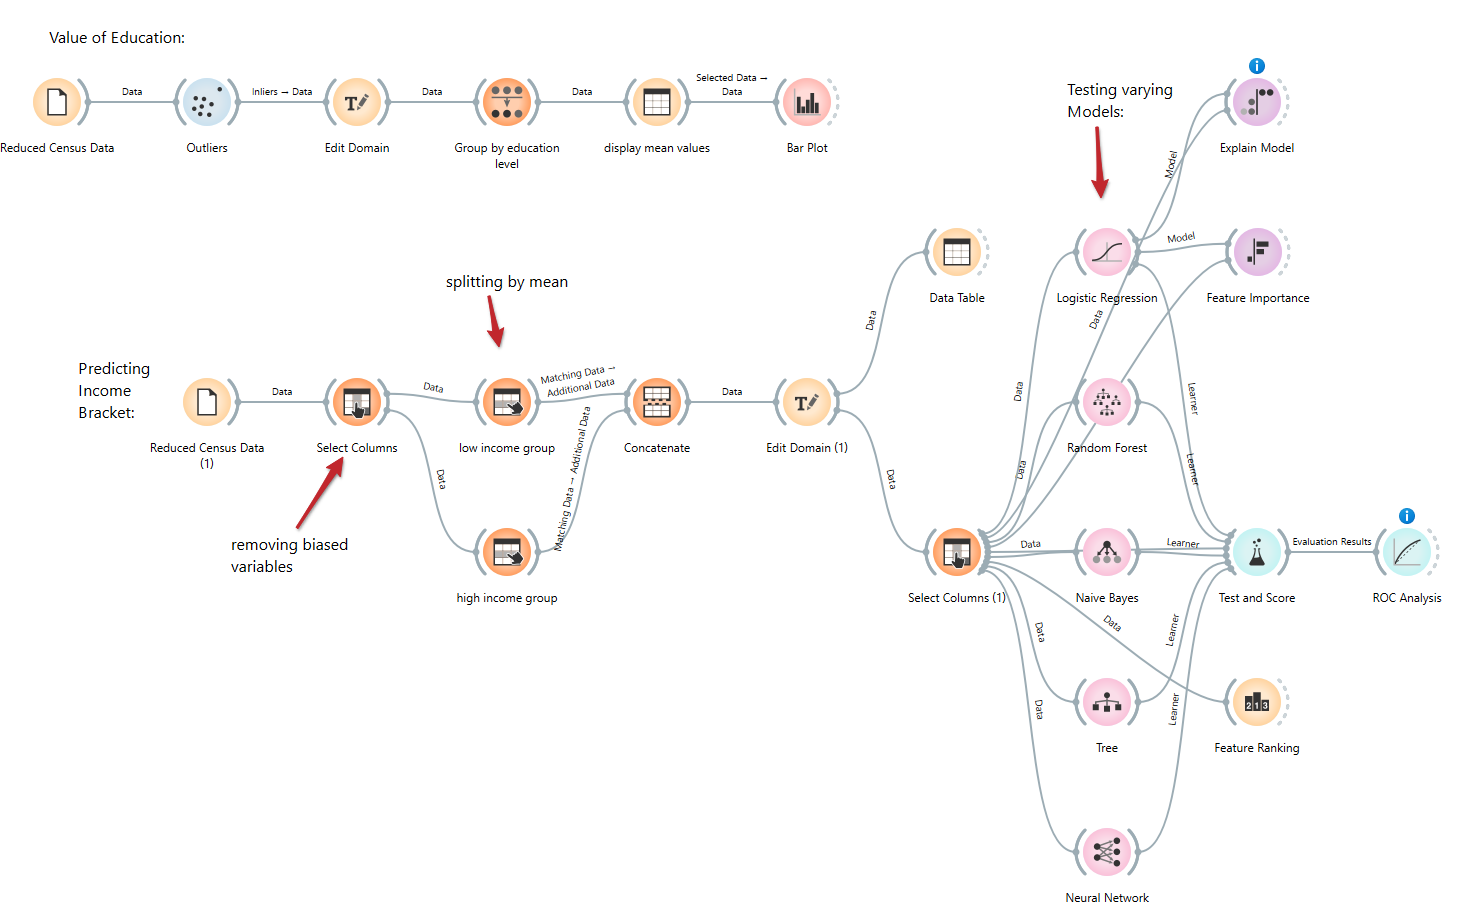
\includegraphics[width=0.9\textwidth]{chapters/part 3 - image/nodes_overview.png}
    \caption{Model training and explainability structure.}
    \label{fig:workflow}
\end{figure}

After removing the \textbf{income} numerics to prevent data leakage, the following results were found:
\begin{figure}[H]
    \centering
    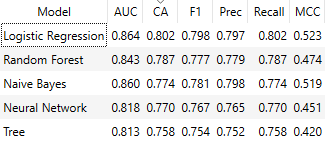
\includegraphics[width=0.7\textwidth]{chapters/part 3 - image/5_model_comparison.png}
    \caption{Model comparisons on determining if someone's income will be high or low}
\end{figure}
\textbf{Logistic Regression} is the winning model with a \texttt{Classification Accuracy} of $80.2\%$ and an \texttt{AUC}
of $0.864$. That a simple model outperforms more complex models (Neural Networks) suggests a strong linear correlation
between the attributes and classification, providing a more generalised model that avoids overfitting.
\begin{figure}[H]
     \centering
     \begin{subfigure}[b]{0.48\textwidth}
         \centering
         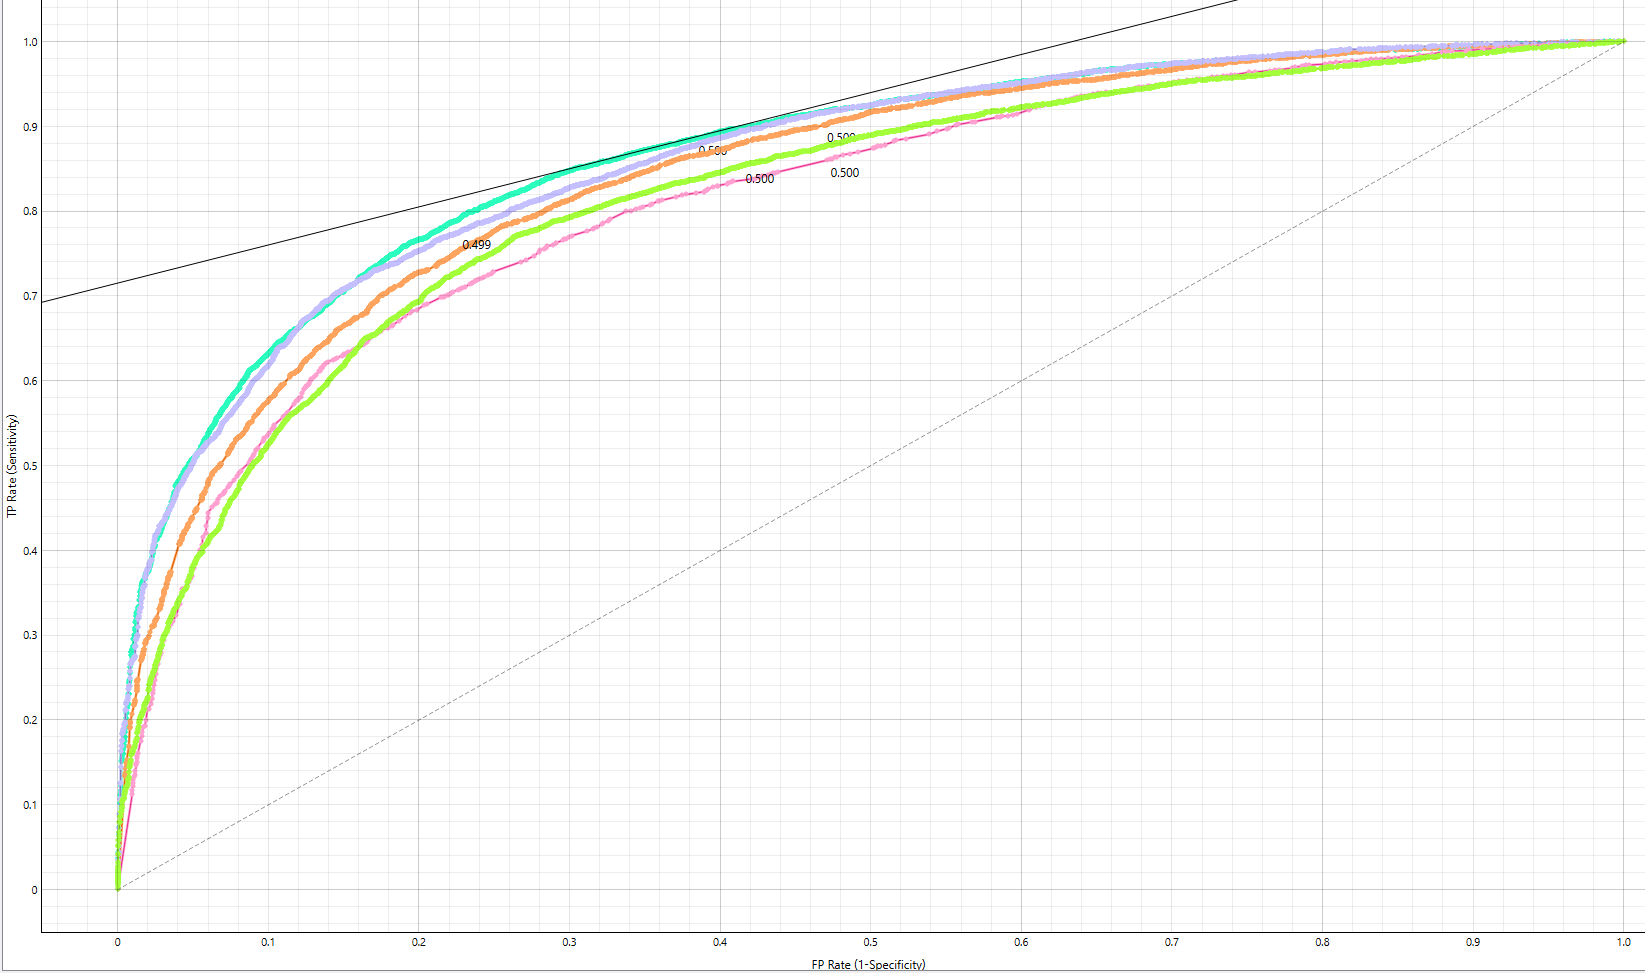
\includegraphics[width=\textwidth]{chapters/part 3 - image/low_income_pred.png}
         \caption{Predictively for Low Income bracket.}
         \label{fig:feature_rank}
     \end{subfigure}
     \hfill
     \begin{subfigure}[b]{0.48\textwidth}
         \centering
         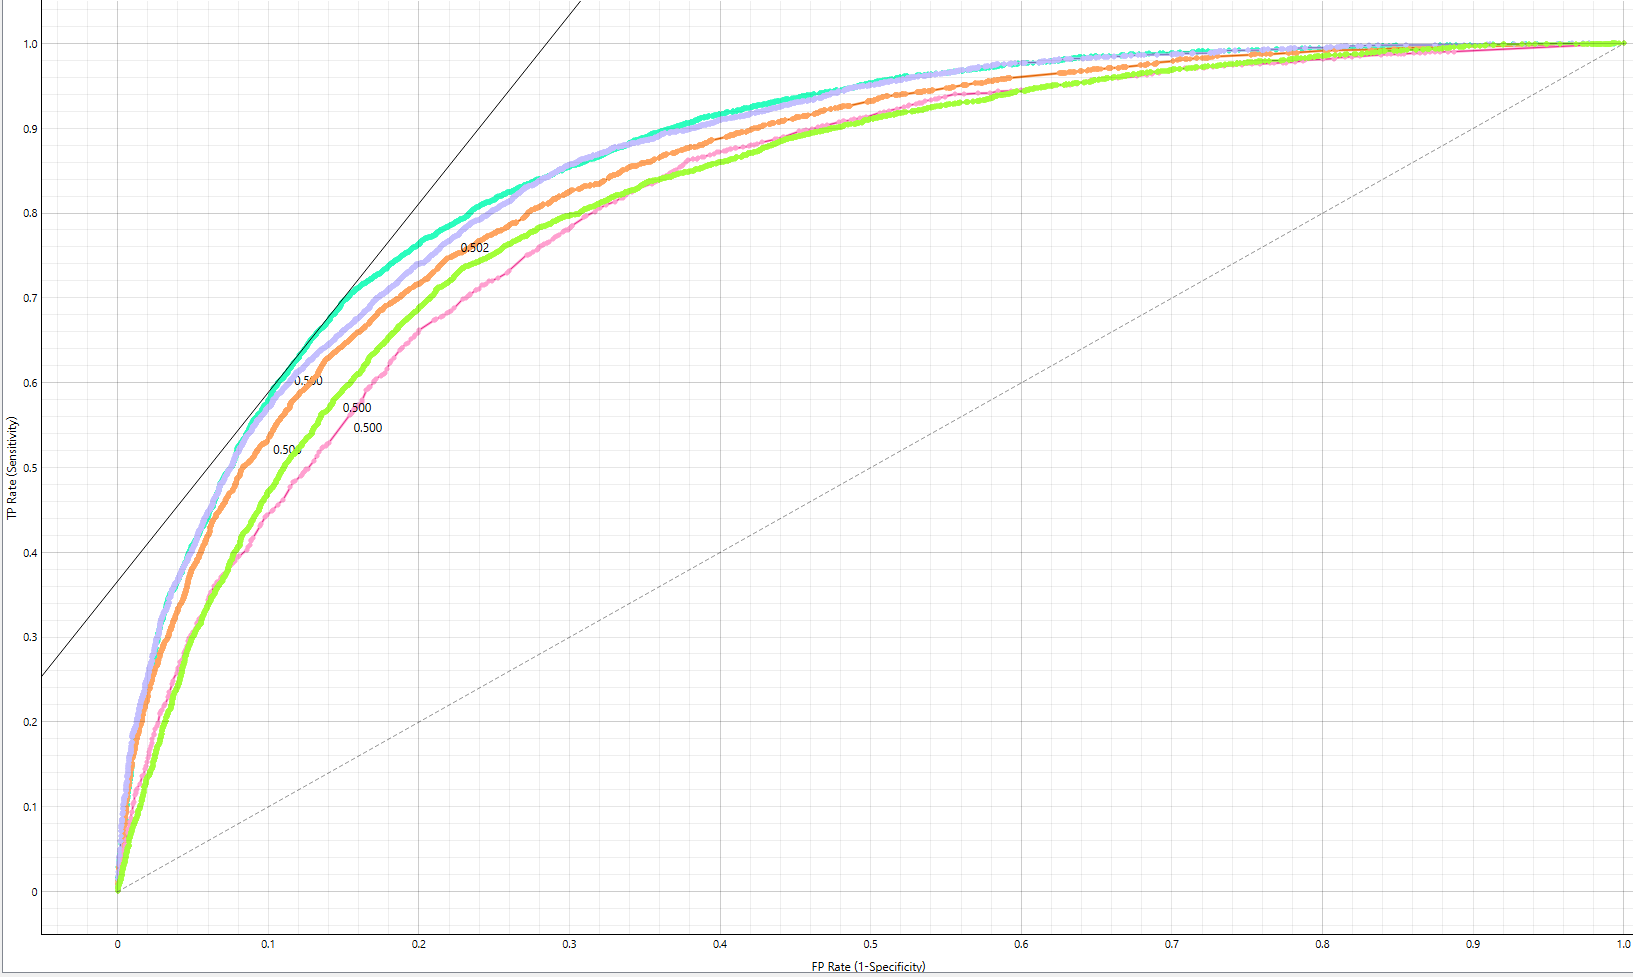
\includegraphics[width=\textwidth]{chapters/part 3 - image/high_income_pred.png}
         \caption{Predictively for High Income bracket.}
         \label{fig:model_comp}
     \end{subfigure}
     \caption{Logistics Regression outperforming for both classifications.}
     \label{fig:side_by_side_comparison}
\end{figure}

\section{Feature Ranking}
\begin{figure}[H]
    \centering
    \begin{subfigure}[b]{0.48\textwidth}
        \centering
        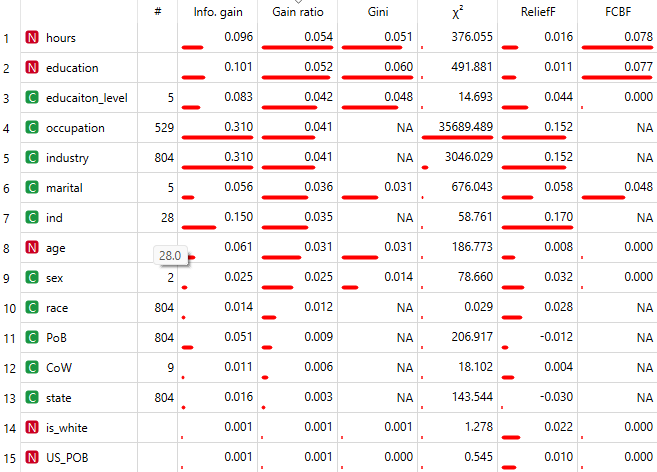
\includegraphics[width=\textwidth]{chapters/part 3 - image/feature_ranking.png}
        \caption{Feature ranking for predicting income low/high}
        \label{fig:feature_rank}
    \end{subfigure}
    \hfill
    \begin{subfigure}[b]{0.48\textwidth}
        \centering
        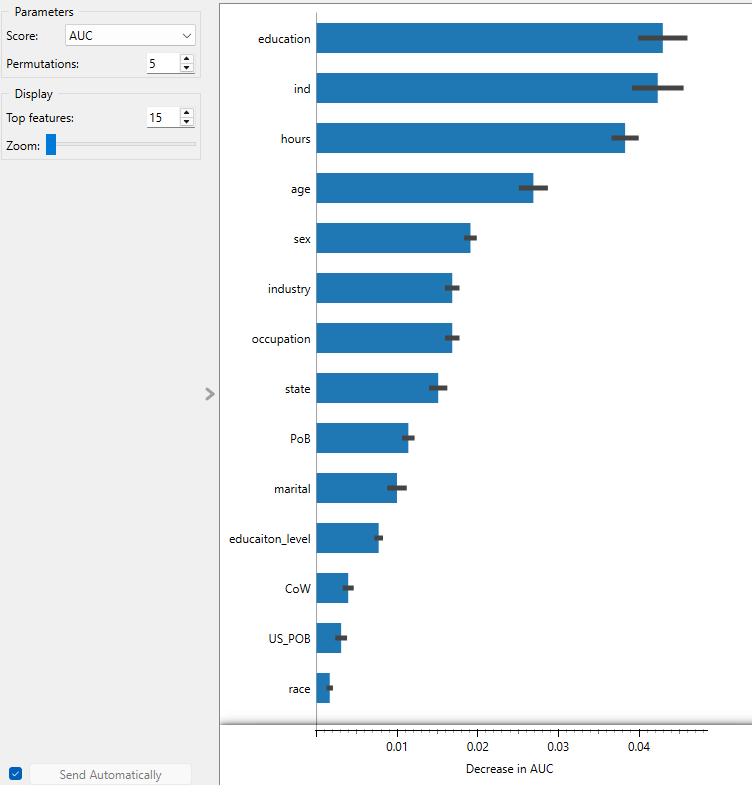
\includegraphics[width=\textwidth]{chapters/part 3 - image/lr_ranks.png} 
        \caption{Model-based feature importance}
        \label{fig:model_explain}
    \end{subfigure}
    \caption{Comparison of data-driven feature ranking and model explainability.}
    \label{fig:side_by_side}
\end{figure}

\textbf{Occupation} and \textbf{industry} yield the highest Information Gain (0.310), indicating primary predictive power. However,
the high granularity of \texttt{industry} suggests potential overfitting; \texttt{ind} (the third most influential feature) is used
to reduce this effect. Conversely, demographic features like \textbf{US\_Place-of-Birth} show negligible influence. The alignment
between these rankings and Figure \ref{fig:model_explain} confirms the model is transparent, making predictions based on initial data
rather than unintuitive correlations. However, \textbf{occupation} lost influence in the regression model despite its high initial
rank; likely due to its \textbf{high cardinality}, creating noise.

\section{Prediction Influence}
\begin{figure}[H]
    \centering
    \begin{subfigure}[b]{0.48\textwidth}
        \centering
        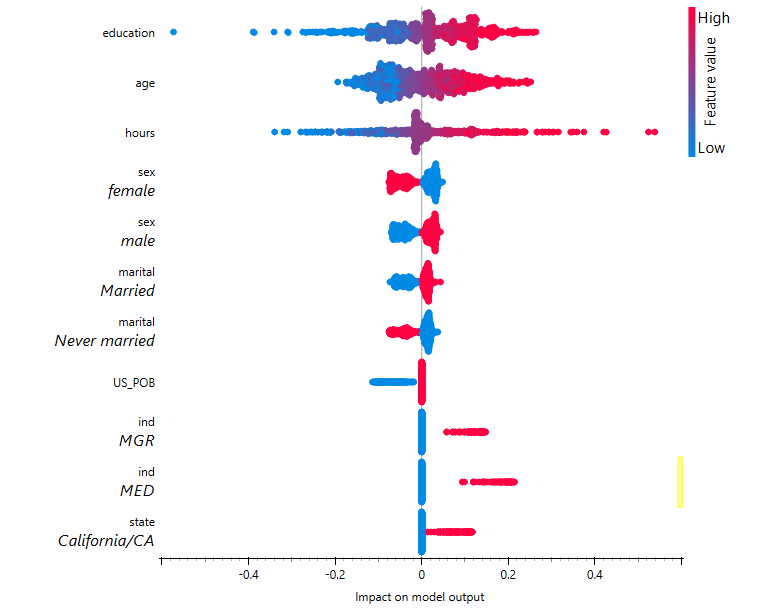
\includegraphics[width=\textwidth]{chapters/part 3 - image/top_influences.png}
        \caption{Global Feature Importance (Beeswarm)}
        \label{fig:global_shap}
    \end{subfigure}
    \hfill
    % Second Image: Local Prediction (Waterfall)
    \begin{subfigure}[b]{0.48\textwidth}
        \centering
        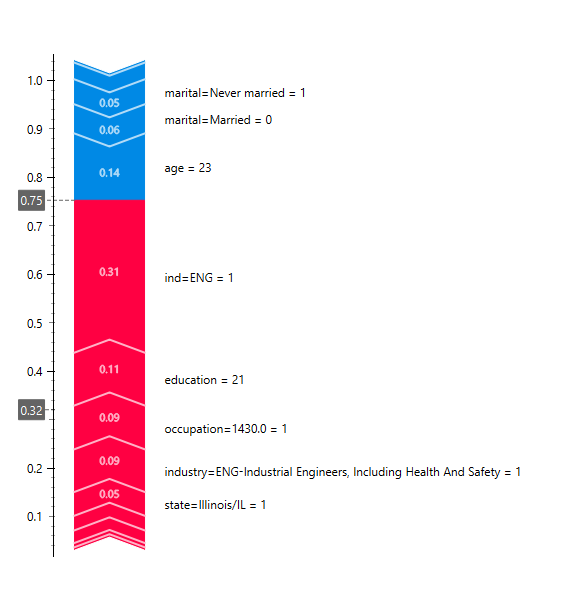
\includegraphics[width=\textwidth]{chapters/part 3 - image/SHAP_spec.png}
        \caption{Local Prediction Explanation (Waterfall)}
        \label{fig:local_shap}
    \end{subfigure}
    
    \caption{Model explainability using SHAP: (a) shows the overall impact of features across the dataset, while (b) illustrates the specific
    feature contributions for a single high-income prediction.}
    \label{fig:prediction_influences}
\end{figure}
The SHAP summary plot (Figure \ref{fig:global_shap}) illustrates the directional influence of key features. Higher values
of education, age and working hours (red) increase the probability of a \texttt{high income} classification. Conversely, being
\texttt{female} pushes the classification towards the \texttt{low income} (represented by blue). Industry sectors such as
MGR(managerial) or MED(medical), also suggest a higher income, validating the importance of professional sector over geographical
location.
The SHAP waterfall plot (Figure \ref{fig:local_shap}) provides a granular view on how features interact to a classification. This
shows how those in the \texttt{Engineering} industry ($+0.31$) and \texttt{higher} education ($+0.11$) push the class to \texttt{high income} despite items
like age pushing it down. Showing how professional and educational background successfully override the demographic disadvantage, puhsing
the prediction above the $0.32$ baseline.